\documentclass[11pt]{book}

%%%%%%%%%%%%%%Include Packages%%%%%%%%%%%%%%%%%%%%%%%%%%
\usepackage{xcolor}
\usepackage{mathtools}
\usepackage[a4paper, total={6in, 8in}, margin=1in]{geometry}
\usepackage{amsmath}
\usepackage{amssymb}
\usepackage{paralist}
\usepackage{rsfso}
\usepackage{amsthm}
\usepackage{wasysym}
\usepackage[inline]{enumitem}   
\usepackage{hyperref}
\usepackage{tocloft}
\usepackage{wrapfig}
\usepackage{titlesec}
\usepackage{colortbl}
\usepackage{stackengine} 
\usepackage{csvsimple}
\usepackage{listings}
%%%%%%%%%%%%%%%%%%%%%%%%%%%%%%%%%%%%%%%%%%%%%%%%%%%%%%%%



%%%%%%%%%%%%%%%Code%%%%%%%%%%%%%%%%%%%%%%%%%%%%%%%%%%%%%
\definecolor{codegreen}{rgb}{0,0.6,0}
\definecolor{codegray}{rgb}{0.5,0.5,0.5}
\definecolor{codepurple}{rgb}{0.58,0,0.82}
\definecolor{backcolour}{rgb}{0.95,0.95,0.92}

\lstdefinestyle{mystyle}{
    backgroundcolor=\color{backcolour},   
    commentstyle=\color{codegreen},
    keywordstyle=\color{magenta},
    numberstyle=\tiny\color{codegray},
    stringstyle=\color{codepurple},
    basicstyle=\ttfamily\footnotesize,
    breakatwhitespace=false,         
    breaklines=true,                 
    captionpos=b,                    
    keepspaces=true,                 
    numbers=left,                    
    numbersep=5pt,                  
    showspaces=false,                
    showstringspaces=false,
    showtabs=false,                  
    tabsize=2
}
%%%%%%%%%%%%%%%%%%%%%%%%%%%%%%%%%%%%%%%%%%%%%%%%%%%%%%%%




%%%%%%%%%%%%%%%Chapter Setting%%%%%%%%%%%%%%%%%%%%%%%%%%
\definecolor{gray75}{gray}{0.75}
\newcommand{\hsp}{\hspace{20pt}}
\titleformat{\chapter}[hang]{\Huge\bfseries}{\thechapter\hsp\textcolor{gray75}{$\mid$}\hsp}{0pt}{\Huge\bfseries}
%%%%%%%%%%%%%%%%%%%%%%%%%%%%%%%%%%%%%%%%%%%%%%%%%%%%%%%%

%%%%%%%%%%%%%%%%%Theorem environments%%%%%%%%%%%%%%%%%%%
\newtheoremstyle{break}
  {\topsep}{\topsep}%
  {\itshape}{}%
  {\bfseries}{}%
  {\newline}{}%
\theoremstyle{break}
\theoremstyle{break}
\newtheorem{axiom}{Axiom}
\newtheorem{thm}{Theorem}[section]
\renewcommand{\thethm}{\arabic{section}.\arabic{thm}}
\newtheorem{lem}{Lemma}[thm]
\newtheorem{prop}[lem]{Proposition}
\newtheorem{corL}{Corollary}[lem]
\newtheorem{corT}[lem]{Corollary}
\newtheorem{defn}{Definition}[corL]
\newenvironment{indEnv}[1][Proof]
  {\proof[#1]\leftskip=1cm\rightskip=1cm}
  {\endproof}
%%%%%%%%%%%%%%%%%%%%%%%%%%%%%%%%%%%%%%%%%%%%%%%%%%%%%%


%%%%%%%%%%%%%%%%%%%%%%%Integral%%%%%%%%%%%%%%%%%%%%%%%
\def\upint{\mathchoice%
    {\mkern13mu\overline{\vphantom{\intop}\mkern7mu}\mkern-20mu}%
    {\mkern7mu\overline{\vphantom{\intop}\mkern7mu}\mkern-14mu}%
    {\mkern7mu\overline{\vphantom{\intop}\mkern7mu}\mkern-14mu}%
    {\mkern7mu\overline{\vphantom{\intop}\mkern7mu}\mkern-14mu}%
  \int}
\def\lowint{\mkern3mu\underline{\vphantom{\intop}\mkern7mu}\mkern-10mu\int}
%%%%%%%%%%%%%%%%%%%%%%%%%%%%%%%%%%%%%%%%%%%%%%%%%%%%%%



\newcommand{\R}{\mathbb{R}}
\newcommand{\N}{\mathbb{N}}
\newcommand{\Z}{\mathbb{Z}}
\newcommand{\Q}{\mathbb{Q}}
\newcommand{\C}{\mathbb{C}}
\newcommand{\T}{\mathcal{T}}
\newcommand{\M}{\mathcal{M}}
\newcommand{\Symm}{\text{Symm}}
\newcommand{\Alt}{\text{Alt}}
\newcommand{\Int}{\text{Int}}
\newcommand{\Bd}{\text{Bd}}
\newcommand{\Power}{\mathcal{P}}
\newcommand{\ee}[1]{\cdot 10^{#1}}
\newcommand{\spa}{\text{span}}
\newcommand{\sgn}{\text{sgn}}
\newcommand{\degr}{\text{deg}}
\newcommand{\pd}{\partial}
\newcommand{\that}[1]{\widetilde{#1}}
\newcommand{\lr}[1]{\left(#1\right)}
\newcommand{\vmat}[1]{\begin{vmatrix} #1 \end{vmatrix}}
\newcommand{\bmat}[1]{\begin{bmatrix} #1 \end{bmatrix}}
\newcommand{\pmat}[1]{\begin{pmatrix} #1 \end{pmatrix}}
\newcommand{\rref}{\xrightarrow{\text{row\ reduce}}}
\newcommand{\txtarrow}[1]{\xrightarrow{\text{#1}}}
\newcommand\oast{\stackMath\mathbin{\stackinset{c}{0ex}{c}{0ex}{\ast}{\Circle}}}


\newcommand{\note}{\color{red}Note: \color{black}}
\newcommand{\remark}{\color{blue}Remark: \color{black}}
\newcommand{\example}{\color{green}Example: \color{black}}
\newcommand{\exercise}{\color{green}Exercise: \color{black}}

%%%%%%%%%%%%%%%%%%%%%%Roman Number%%%%%%%%%%%%%%%%%%%%%%%
\makeatletter
\newcommand*{\rom}[1]{\expandafter\@slowromancap\romannumeral #1@}
\makeatother
%%%%%%%%%%%%%%%%%%%%%%%%%%%%%%%%%%%%%%%%%%%%%%%%%%%%%%%%%

%%%%%%%%%%%%table of contents%%%%%%%%%%%%%%%%%%%%%%%%%%%%
\setlength{\cftchapindent}{0em}
\cftsetindents{section}{2em}{3em}

\renewcommand\cfttoctitlefont{\hfill\huge\bfseries}
\renewcommand\cftaftertoctitle{\hfill\mbox{}}

\setcounter{tocdepth}{2}
%%%%%%%%%%%%%%%%%%%%%%%%%%%%%%%%%%%%%%%%%%%%%%%%%%%%%%%%%


%%%%%%%%%%%%%%%%%%%%%Footnotes%%%%%%%%%%%%%%%%%%%%%%%%%%%
\newcommand\blfootnote[1]{%
  \begingroup
  \renewcommand\thefootnote{}\footnote{#1}%
  \addtocounter{footnote}{-1}%
  \endgroup
}
%%%%%%%%%%%%%%%%%%%%%%%%%%%%%%%%%%%%%%%%%%%%%%%%%%%%%%%%%

%%%%%%%%%%%%%%%%%%%%%Section%%%%%%%%%%%%%%%%%%%%%%%%%%%%%
\makeatletter
\def\@seccntformat#1{%
  \expandafter\ifx\csname c@#1\endcsname\c@section\else
  \csname the#1\endcsname\quad
  \fi}
\makeatother
%%%%%%%%%%%%%%%%%%%%%%%%%%%%%%%%%%%%%%%%%%%%%%%%%%%%%%%%%

%%%%%%%%%%%%%%%%%%%%%%%%%%%%%%%%%%%Enumerate%%%%%%%%%%%%%%
\makeatletter
% This command ignores the optional argument 
% for itemize and enumerate lists
\newcommand{\inlineitem}[1][]{%
\ifnum\enit@type=\tw@
    {\descriptionlabel{#1}}
  \hspace{\labelsep}%
\else
  \ifnum\enit@type=\z@
       \refstepcounter{\@listctr}\fi
    \quad\@itemlabel\hspace{\labelsep}%
\fi}
\makeatother
\parindent=0pt
%%%%%%%%%%%%%%%%%%%%%%%%%%%%%%%%%%%%%%%%%%%%%%%%%%%%%%%%%%


\begin{document}

	\begin{titlepage}
		\begin{center}
			\vspace*{1cm}
			\Huge \color{red}
				\textbf{Lab 5 Report}\\
			\vspace{0.5cm}			
			\Large \color{black}
				Math 391 - Introduction to Modern Physics Lab\\
				Professor Wayne Lau\\	
				University of Michigan\\
			\vspace{3cm}

			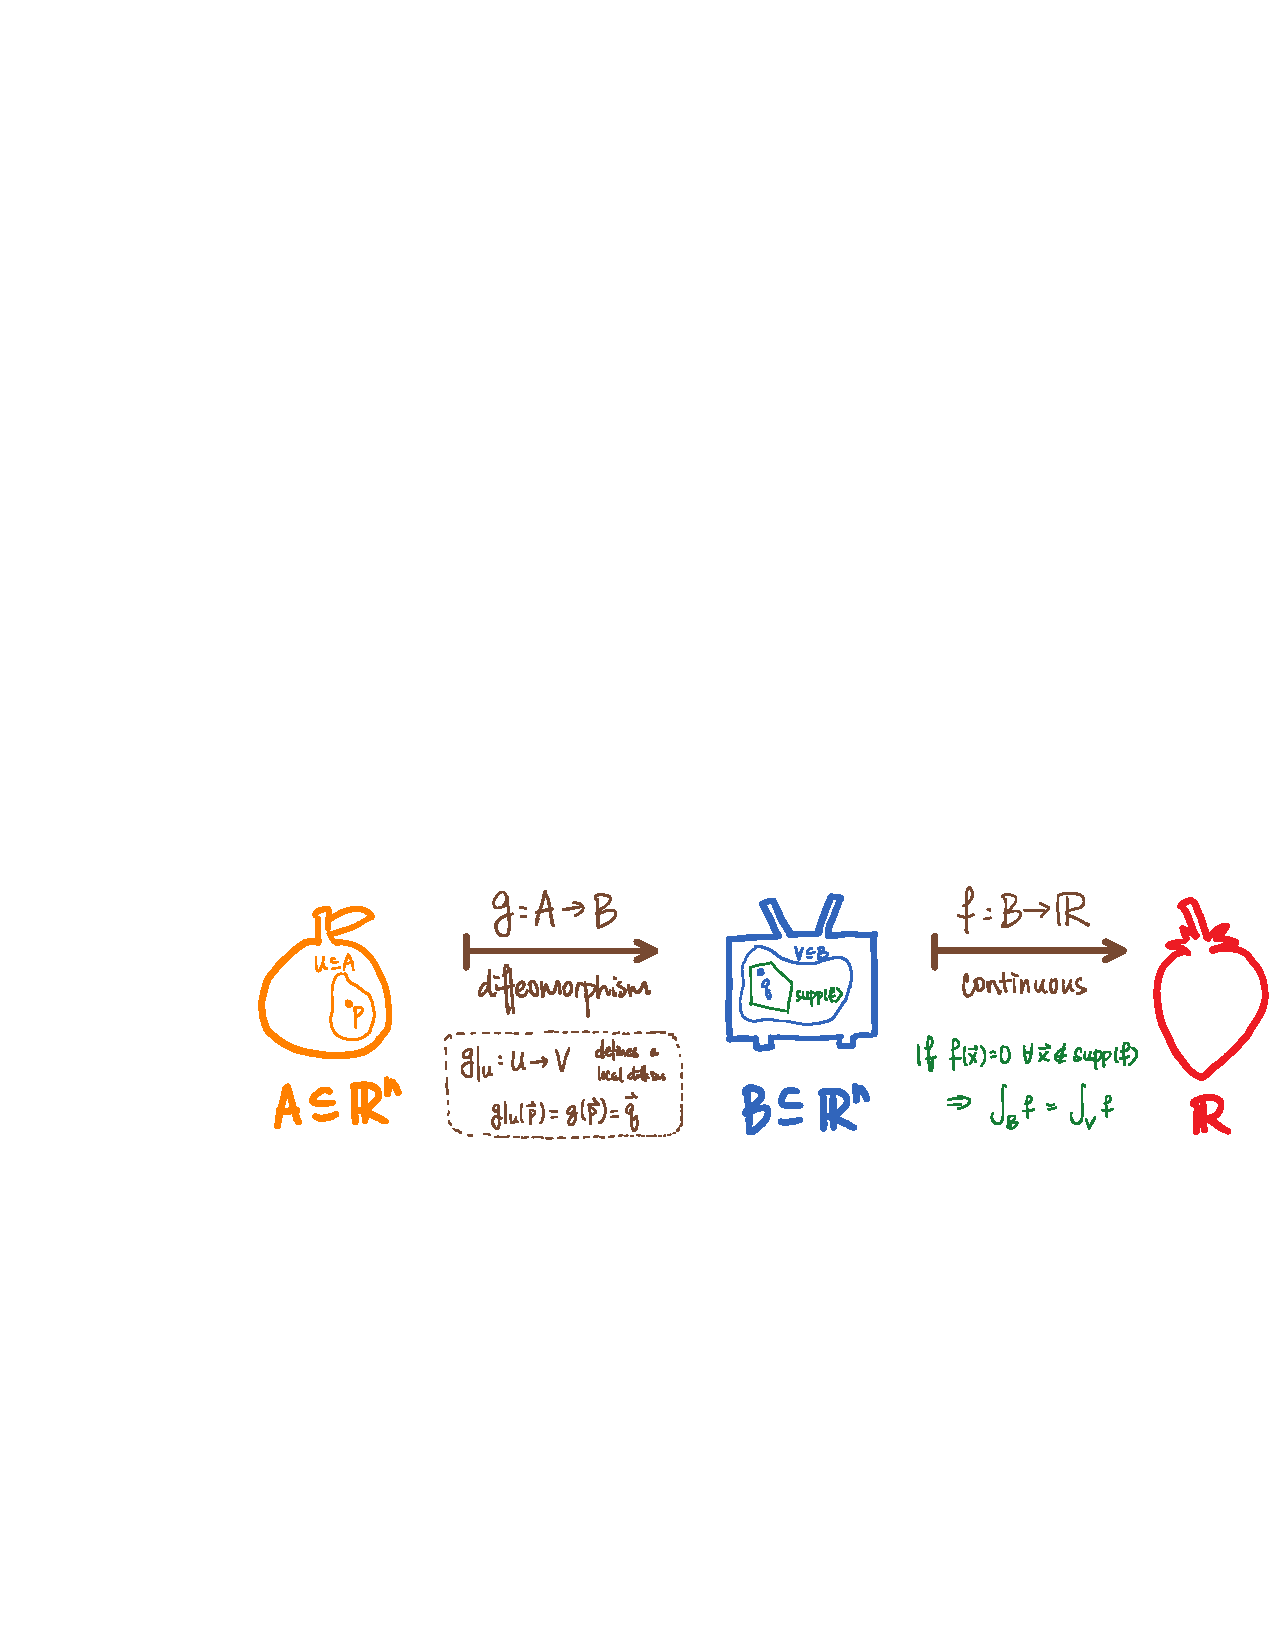
\includegraphics[scale=0.8]{cor13.4.pdf}\\
			\color{gray}The Change of Variable Theorem\color{black}
			
			
			\vspace{5cm}
			\LARGE
				\textbf{Jinyan Miao}\\
				\hfill\break
				\LARGE Fall 2022\\
			\vspace{1cm}

		\vspace*{\fill}
		\end{center}			
	\end{titlepage}


\newpage
\tableofcontents
\addtocontents{toc}{~\hfill\textbf{Page}\par}


\setcounter{chapter}{3}
\chapter*{Lab 5 - Crystal Structure Measuring}
\section{Introduction}
In quantum mechanics, particles also have wave properties, and the wavelength of a particle of non-relativistic momentum $p$ is given by the de Broglie relation:
\begin{align*}
\lambda = \frac{h}{p}
\end{align*}
where $h$ is the Planck's constant. In Lab 5 of Physics 391, we verify the de Broglie relation and make measurements of the inter-atomic distance in a crystal structure.\\


We use a cathode ray tube (manufactured by Leybold Didactic) with a graphite crystal target that can be used to produce a diffraction pattern on the screen. In the cathode ray tube, the electrons are accelerated by a high voltage $V$, such that the accelerated electrons have de Broglie's wavelength given by the following:
\begin{align}
\lambda = \frac{h}{\sqrt{2eVm}}
\end{align}

The vertices of the unit cell in the crystal structure are atoms, and the size of the unit cell is related to the inter-atomic spacings, or the lattice constant. In our experiment, the graphite crystal has a layered, planar structure. The geometry of the structure is shown as the following:
\begin{center}
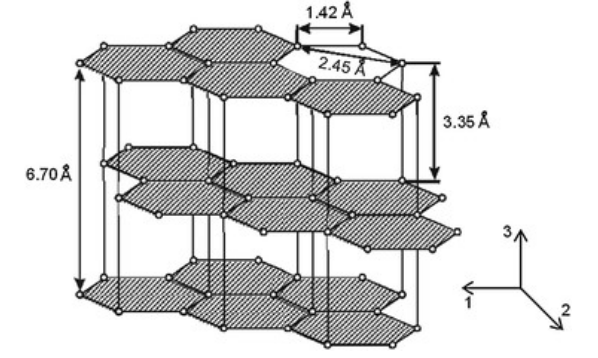
\includegraphics[scale=0.69]{structure1.png}
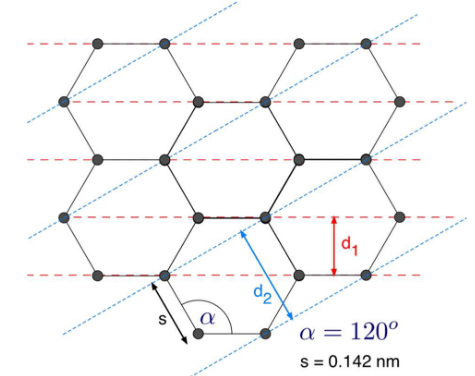
\includegraphics[scale=0.69]{structure2.png}\\
\color{gray} Figure 1 and 2 from Physics 391 Lab Manual, Experiment 5.\color{black}
\end{center}
Here $d_1$ and $d_2$ are calculated to be the followings:
\begin{align*}
d_1 &= 0.142\cdot \sin(\pi/3)\cdot 10^{-9} \, m = 1.2298\cdot 10^{-10} \, m\\
d_2 &= 0.142\cdot (\sin(\pi/6)+1)\cdot 10^{-9} \, m = 2.1300\cdot 10^{-10}\, m
\end{align*}
We can think of the regular arrays in the crystal in terms of planes of atoms, as the beam of electrons reaches one of the planes, the beam will either pass through the plane and reach the next plane, or get reflected as if by a simple plane mirror. The sum of the reflection from a large number of parallel planes all separated by the same distance will produce a constructive interference pattern when the angle between the beam and the surface satisfies the Bragg's condition:
\begin{align*}
2d\sin(\theta) = n\lambda \qquad \forall n \in \N
\end{align*}

As a result, a beam of electrons incident on the sample target will find many small crystal domains oriented at the correct Bragg's angle for the Bragg's wavelength of the electrons, and, via the Bragg's condition and the simple geometry in our setup, the locus of the constructively reflected wave will be a cone with half-angle equal to twice the Bragg's angle. Hence the diffraction maximum traces a circle in the projection plane. Assuming the circle has a diameter $D$ and the distance between the target and the screen is $L$, then the half-angle $\alpha$ of the cone is given by the following:
\begin{align}
\tan(\alpha) = \frac{D}{2L}
\end{align}
and the Bragg's angle is given by $\theta = \alpha /2$. 

\hfill\break
\section{Experimental setup} In our setup, $L = 0.135\, m$, the target is crystalline in tiny regions, so the powder diffraction pattern results in a pair of rings around a central spot on the luminescent screen. In this text, we will call the two rings as inner ring and outer ring.\\

A Mylar film is used to measure the diameters of the two rings. The Mylar film is attached on the screen. For each ring, we draw two perpendicular lines through the center of the ring, mark the intersection between the lines and the ring, measure the distance between the marks on each line, and take the average of the two to get a diameter of the ring. We repeat this procedure for different voltages that accelerates the electrons, starting from $5\, kV$ to $2\, kV$, in steps of $0.5\, kV$. \\

Via (3.2), we can calculate the Bragg's angles for each ring and each voltage:
\begin{align}
\theta = \frac{1}{2}\tan^{-1}\left( \frac{D}{2L}\right)
\end{align}
and via (3.1), the Bragg's angle also satisfies the following:
\begin{align}
\sin(\theta) = \frac{h}{2d\sqrt{2emV}}
\end{align}
According to (3.4) we expect to see a linear relationship between $\sin(\theta)$ and $V^{1/2}$, and the slope of such linear relationship is characterized by the distance $d$ between the lattice. For the inner ring, $d$ should corresponds to $d_2$ as computed above, and for the outer ring, $d$ should corresponds to $d_1$ as computed above. 
 
\newpage
\section{Visualizing the data}
First, we present our data in the following plots for $\sin(\theta)$ versus $V^{1/2}$:
\begin{center}
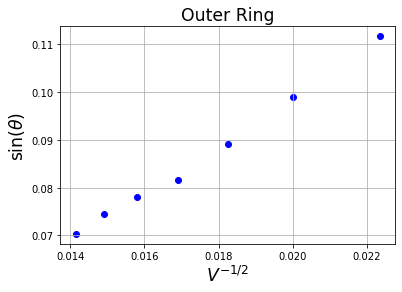
\includegraphics[scale=0.55]{Or.png} 
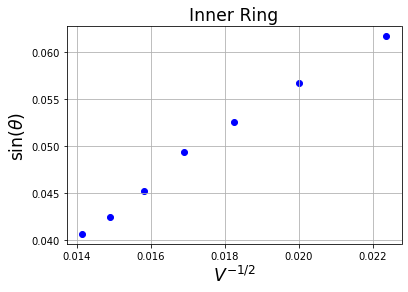
\includegraphics[scale=0.55]{Ir.png}\\
${}$\qquad\quad Figure 2a \qquad\qquad\qquad\qquad\qquad\qquad\qquad\qquad Figure 2b
\end{center}
\hfill\break

\section{Analyzing the data}
We then fit our data via (3.4):
\begin{center}
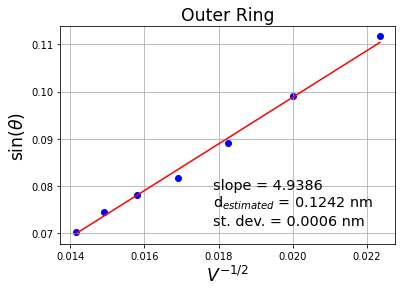
\includegraphics[scale=0.55]{Of.png} 
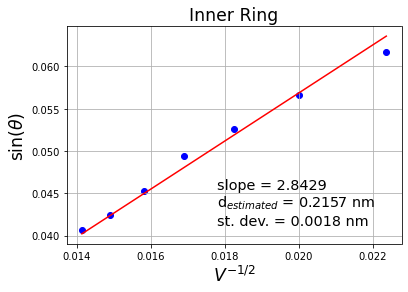
\includegraphics[scale=0.55]{If.png}\\
${}$\qquad\quad Figure 1a \qquad\qquad\qquad\qquad\qquad\qquad\qquad\qquad Figure 1b
\end{center}
where $d_{\text{estimated}}$ is computed by the following, with $s$ being the slope of the linear fit:
\begin{align*}
d_{\text{estimated}} = \frac{h}{2s\sqrt{2em}}
\end{align*}
According to error propagation, the standard deviation of $d_{estimated}$, denoted as $\sigma_d$ is calculated from the standard deviation of $s$, denoted as $\sigma_s$, and $\sigma_s$ is obtained from the linear fit:
\begin{align*}
\sigma_d = \frac{\sigma_s}{s}\cdot d
\end{align*}
For the outer ring, the estimated spacing of the lattice is given by $0.1242\, nm$, with a standard deviation of $0.0006\, nm$. The theoretical value for the spacing, in this case, is $0.1230 \, nm$. Here we can calculate the following:
\begin{align*}
\frac{|(0.1242\, nm) - (0.1230\,nm)|}{(0.0006\, nm)} =2 
\end{align*}
so we see that the theoretical value $d_1$ falls within $3$ standard deviation from the estimated $d_1$. This implies that the theoretical value $d_1$ is statistically well-predicted by our experimental results, or in other words, our experimental result gives a good approximation for $d_1$.\\


For the inner ring, the estimated spacing of the lattice is given by $0.2157\, nm$, with a standard deviation of $0.0018\, nm$. The theoretical value for the spacing, in this case, is $0.2130 \, nm$. Here we can calculate the following:
\begin{align*}
\frac{|(0.2157\, nm) - (0.2130\,nm)|}{(0.0018\, nm)} =1.5 
\end{align*}
so we see that the theoretical value $d_2$ also falls within $3$ standard deviation from the estimated $d_2$. This implies that the theoretical value $d_2$ is statistically well-predicted by our experimental results, or in other words, our experimental result gives a good approximation for $d_2$.\\


The result of this experiment depends very much on the wave nature of the electrons. In this experiment, we have also verified the de Broglie relation as we are able to observe the constructive interference of the electron beams characterized by the bright rings on the screen. By using the diffraction property of an electron beam, we can determine the spacing of the atoms in the crystal structure. Note that, the interlayer spacing ($3.35 \cdot 10^{-10}\, m$) for the crystal structure does not result in a third ring being observed on the screen because the diameter of such ring will be relatively small:
\begin{align*}
\theta = \sin^{-1}\left(\frac{h}{2d \sqrt{2em V}}\right) \qquad \Rightarrow \qquad D = 2\cdot L \cdot \tan(2\theta)\approx 1.4\, cm \tag{$V=5\, kV$}
\end{align*}
and also because the wavelengths of the accelerated electron are not comparable to interlayer spacings, which makes the Bragg's condition for electron diffraction not applicable:
\begin{align*}
\lambda_e = \frac{h}{\sqrt{2e Vm}} \approx 2.7425\cdot 10^{-11} m \ll 3.35 \cdot 10^{-10}\, m \tag{$V = 2\, kV$}
\end{align*}


\hfill\break
\hfill\break
\section{Summary}
In this Lab, we determined the spacing between the atoms in the graphite crystal structure by using the diffraction property of the electrons beam. The analysis is based on de Broglie's wavelength of the accelerated electrons and the Bragg's condition applied to the crystal structure that produces a constructive interference pattern on the screen. In our experiment, the parameters $d_1$ and $d_2$, which characterize the geometry of the lattice, is found to be $0.1242\pm 0.0006\, nm$ and $0.2157\pm 0.0018\, nm$, respectively. Compared to the theoretical results of $d_1$ and $d_2$, we conclude that our experimental results are statistically well-predicted. 


\newpage
\section{Jinyan's Topic for the Presentation}
\subsection{PT-symmetry in optical based system}
Symmetry breaking of photonic-based PT-symmetric systems have been demonstrated to generate unexpected physical phenomena while useful application in lasers and sensors. When a photonic-based PT-symmetric system is in the broken PT-symmetric phase, the system has a complex energy spectrum. Former studies, such that alpha decay introduced by George Gamow and non-Hermitian complex potential introduced by Feshbach, Porter and Weisskopf, have shown that the imaginary part of the energies of a system does have physical meaning. To demonstrate conventional photonic-based PT-symmetry, many others have studied the system of coupled photonic components. In the followings we will first review some basic properties of the coupled two-photinic components system, then we will couple the two-component system with an exciton to get a new PT-symmetric system and discuss some of its numeric and analytic results.

\subsection{Coupled two-photonic components system}
Consider a coupled two-photonic components system with a coupling constant $C > 0$, each has energy $E$ one with gain $\gamma > 0$ and the other one with loss $-\gamma$. The Hamiltonian of this system is given by:
\begin{align*}
\mathcal{H } = \bmat{E+i\gamma & C \\  C & E - i\gamma}
\end{align*}
By simple computation, the eigen-energies of this system is given by the followings:
\begin{align*}
\lambda_1 = E + \sqrt{C^2 -\gamma^2} \qquad\qquad\qquad \lambda_2 = E - \sqrt{C^2 - \gamma^2}
\end{align*}
Here we see that:
\begin{align*}
\begin{cases}
C > \gamma & \mathcal{H} \text{ is in unbroken PT-symmetric phase} \\
C = \gamma & \text{Exceptional point occurs} \\
C < \gamma & \mathcal{H} \text{ is in broken PT-symmetric phase}
\end{cases}
\end{align*}
We can also compute the analytic eigensolutions of the system described by $\mathcal{H}$. \\

For $\lambda_1$, the eigensolution is given by the following:
\begin{align*}
\left|\psi\right>_1 = \bmat{m \\  \left( \frac{\sqrt{C^2 - \gamma^2}}{C}-\frac{\gamma}{C}\, i\right)\, m }
\end{align*}
For $\lambda_2$, the eigensolution is given by the following:
\begin{align*}
\left|\psi\right>_2 = \bmat{m \\  \left(- \frac{\sqrt{C^2 - \gamma^2}}{C}-\frac{\gamma}{C} \, i \right)\, m}
\end{align*}
where $m\in \C$ is a constant that is used to normalize the eigensolution such that $\langle\psi |\psi\rangle = 1$. \\

We claim that, for system like the $2\times 2$ Hamiltonian 
$\mathcal{H}$ described above, if the system has nondegenerate spectrum,  the eigenvalues are real if and only if the eigensolutions $ \left|\psi\right>$ are invariant under the PT operator up to a phase factor $\lambda$, that is, we have:
\begin{align*}
PT \left|\psi\right> = \lambda \left|\psi\right> \qquad \text{with }|\lambda | =1  \tag{in unbroken PT-symmetric phase}
\end{align*}
Mathematically, this statement can be generalized by Theorem 2.1 on next page. Many former studies on PT-symmetric systems, such as \textit{PT-symmetry in optics, by Zyablovsky et al (2014)}, and \textit{PT-symmetric quantum mechanics, by Bender et al (1998)}, have also demonstrated this result, but here we will look further on how this result can be analytically applied to our two-photonic components system.\\

For the two-photonic components system, the time operator $T$ is taking the complex conjugate, and the parity operator $P$ is given by the following matrix:
\begin{align*}
P = \bmat{0 & 1 \\ 1 & 0}
\end{align*}
Hence we can see that:
\begin{align*}
PT \left|\psi\right>_1 = \bmat{\left(\frac{\sqrt{C^2 - \gamma^2}}{C}+\frac{\gamma}{C}i\right)m \\ m} = \left(\frac{\sqrt{C^2 - \gamma^2}}{C}+\frac{\gamma}{C}i\right) \left|\psi\right>_1
\end{align*}
When $\gamma< C$, that is, the system is in unbroken PT-symmetry state, then we have:
\begin{align*}
\left| \frac{\sqrt{C^2 - \gamma^2}}{C}+\frac{\gamma}{C}i \right| = 1 \qquad \text{when }\gamma<C
\end{align*}
it follows that, when we have $\gamma > C$, the system is in broken PT-symmetry state, and we have:
\begin{align*}
\left| \frac{\sqrt{C^2 - \gamma^2}}{C}+\frac{\gamma}{C}i \right| \neq 1 \qquad \text{when }\gamma > C
\end{align*}

\begin{center}
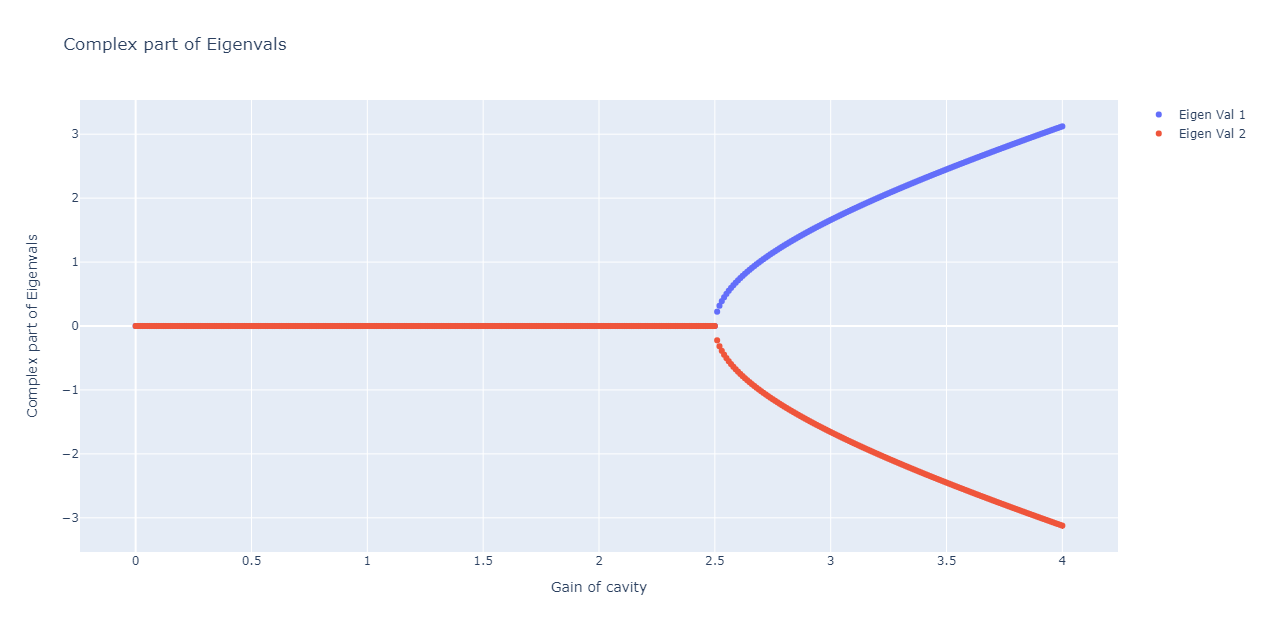
\includegraphics[scale=0.35]{2x2HamComp.png}
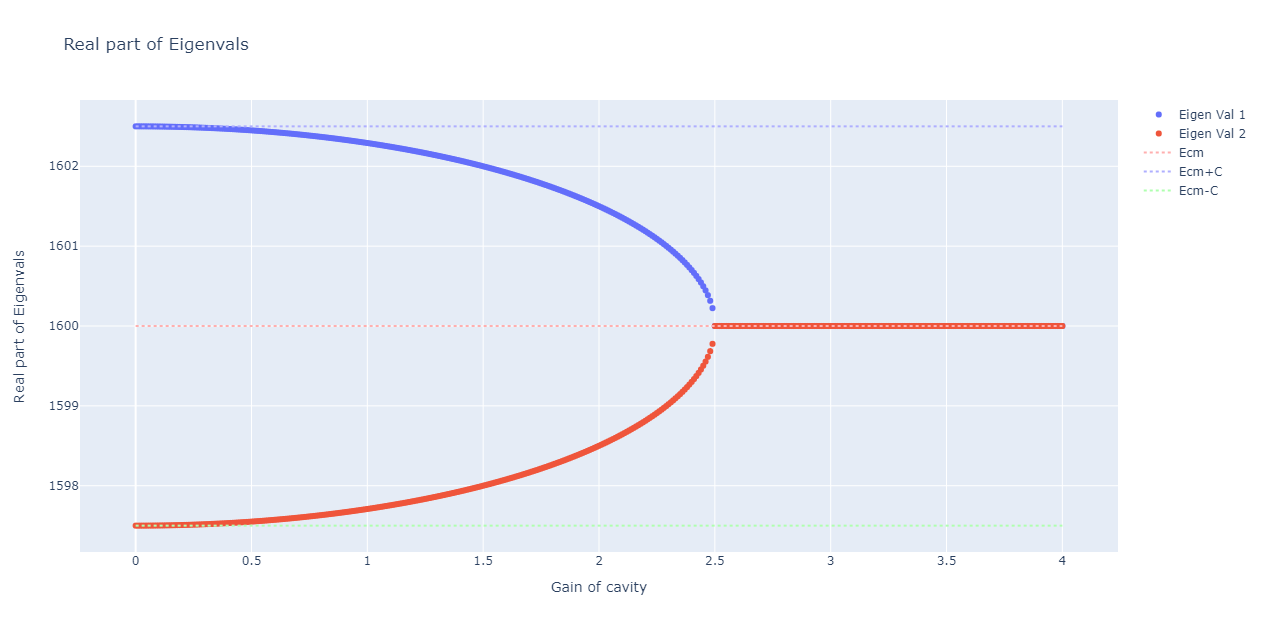
\includegraphics[scale=0.35]{2x2HamReal.png}
\end{center}
\subsection{Exceptional points and re-entrance of unbroken PT-symmetric phase}
\subsection{Sensing in optical based PT-symmetric systems}



\newpage
\section{Experiment Data}
\begin{center}
\begin{tabular}{|c|c|c|c|c|c|}%
\hline
	\textbf{Inner Ring} & &  & & &\\
\hline	
     \bfseries n & \bfseries V &\bfseries D1 &\bfseries D2 & \bfseries average D &\bfseries $\theta_1$ 
    \csvreader[head to column names]{innerRing.csv}{}
    {\\\hline\csvcoli&\csvcolii&\csvcoliii
      &\csvcoliv&\csvcolv&\csvcolvi}\\% specify your coloumns here
\hline  
\end{tabular}  \\
\hfill\break
\hfill\break
\begin{tabular}{|c|c|c|c|c|c|}%
\hline
	\textbf{Outer Ring} & & & & &  \\
\hline	
     \bfseries n & \bfseries V &\bfseries D1 &\bfseries D2 & \bfseries average D &\bfseries $\theta_1$ 
    \csvreader[head to column names]{outerRing.csv}{}
    {\\\hline\csvcoli&\csvcolii&\csvcoliii
      &\csvcoliv&\csvcolv&\csvcolvi}\\% specify your coloumns here
\hline  
\end{tabular} 
\end{center}


\section{Code}
The code for computing statistics of the data sets is attached.
\lstset{style=mystyle}
\lstinputlisting[language=Python]{code.py}


\end{document}